% !TeX document-id = {87432cc9-c386-48dc-9558-b3c42a74a150}
% !TEX encoding = UTF-8
% !TEX TS-program = pdflatex
% !TEX spellcheck = it-IT
%% !TEX root = 
% !BIB TS-program = biber
% Comandi speciali (o righe magiche) trattati come commenti da Latex ma non da 
%editor come Texstudio e Texshop, che si impostano di conseguenza. In ordine:
% dichiara la codifica dei caratteri con cui impostare l'editor (bisogna 
%comunque caricare inputenc con la stessa codifica)
% dichiara il motore di composizione (pdflatex o lualatex)
% attiva il controllo ortografico della lingua del documento
% dichiara la condizione di file principale e di file secondario nei documenti 
%suddivisi in più file
% imposta biber come motore bibliografico

\documentclass[9pt]{extarticle}



% ------------------------------------------------------------------------------
% Packages
% ------------------------------------------------------------------------------
\usepackage[utf8]{inputenc}
\usepackage{graphicx}
\usepackage{amsmath}
\usepackage{amssymb}
\usepackage{amsthm}
\usepackage{hyperref}
\usepackage{titlesec}
\usepackage{parskip}
\usepackage{float}
\usepackage{booktabs}
\usepackage{caption}
\usepackage{blindtext}
\usepackage[table,xcdraw]{xcolor}
\usepackage{enumitem}
% Define a new counter for functional requirements
\newcounter{rf}
\newcommand{\FR}{\refstepcounter{rf}\textbf{FR\therf: }}
% Define a new counter for non-functional requirements
\newcounter{nonfunc}
\newcommand{\NONFUNC}{\refstepcounter{nonfunc}\textbf{NFR\thenonfunc: }}

% ------------------------------------------------------------------------------
% Page setup
% ------------------------------------------------------------------------------
\usepackage{geometry} 
\geometry{a4paper, margin=1in, twoside}
\usepackage{setspace}
\setstretch{1.2}  % Adjust the number as needed
%\doublespacing


% ------------------------------------------------------------------------------
% Referencing
% ------------------------------------------------------------------------------
\usepackage[
	backend=biber,
	citestyle=authoryear,
	bibstyle=authoryear,
	maxcitenames=2,
	maxbibnames=99]{biblatex}
%\addbibresource{references.bib}
%\DeclareNameAlias{sortname}{family-given}
%\setlength\bibitemsep{1em}

% ------------------------------------------------------------------------------
% Code listings
% ------------------------------------------------------------------------------
\usepackage{listings}
\usepackage{xcolor}
\lstdefinestyle{matlabcode}{
	backgroundcolor=\color{gray!10},   
	commentstyle=\color{green!50!black},
	keywordstyle=\color{blue},
	stringstyle=\color{magenta},
	basicstyle=\linespread{1}\footnotesize\ttfamily,
	numberstyle=\tiny,
	breakatwhitespace=false,         
	breaklines=true,                 
	captionpos=t,   
	frame=single,
	keepspaces=true,         
	language=matlab,        
	numbers=none,             
	numbersep=5pt,                  
	showspaces=false,                
	showstringspaces=false,
	showtabs=false,                  
	tabsize=2,
	aboveskip=1em,
	belowskip=1em,
	belowcaptionskip=12pt
}

% ------------------------------------------------------------------------------
% Headers and footers
% ------------------------------------------------------------------------------	
\usepackage{fancyhdr}
\pagestyle{fancy}   
\setlength{\headheight}{14.5pt}
\renewcommand{\headrulewidth}{0.3pt}
%\renewcommand{\chaptermark}[1]{\markboth{\chaptername\ \thechapter.\ #1}{}}
\renewcommand{\sectionmark}[1]{\markright{\thesection.\ #1}}   
\fancyhead[LE,RO]{\rightmark}
\fancyhead[LO,RE]{\leftmark}

% ------------------------------------------------------------------------------
% Title page
% ------------------------------------------------------------------------------

\newcommand{\name}{Togni Roberto}
\newcommand{\projecttitle}{EvenTrento}
\newcommand{\course}{Ingegneria del Software}
\newcommand{\customtitle}{
	\vspace*{1cm}
	\begin{center}
		
\includegraphics[width = 7cm]{images/logo_rosso} \\
		\vspace{1cm}
	\end{center}
	\LARGE{Progetto:}
	\begin{center}
%		\vspace{2cm}
		\textbf{\Huge{\projecttitle}} \\
	\end{center}
	\LARGE{Titolo del documento:}
	\begin{center}
%		\vspace{1cm}
		\textbf{\Huge Descrizione di Progetto} \\
	\end{center}
	\LARGE{Autore:}
	\begin{center}
		%		\vspace{1cm}
		\textbf{\name} \\
	\end{center}
	\vspace{1cm}
	Document Info:
	
	\begingroup
	\setlength{\tabcolsep}{10pt} % Default value: 6pt
	\renewcommand{\arraystretch}{1.5}
	
	\begin{table}[!htb]
		\begin{tabular}{lllll}
			\cline{1-4}
			\cellcolor[HTML]{13315C}{\color[HTML]{FFFFFF} Doc. Name}                         & D1-EvenTrentoDescrizioneProgetto & \multicolumn{1}{l|}{\cellcolor[HTML]{13315C}{\color[HTML]{FFFFFF} Doc. Number}} & \multicolumn{1}{l|}{D1 V0.1} &  \\ \cline{1-4}
			\multicolumn{1}{|l|}{\cellcolor[HTML]{13315C}{\color[HTML]{FFFFFF} Description}} & \multicolumn{3}{l|}{Documento di analisi dei requisiti funzionali, non funzionali e front-end}                                                    &  \\ \cline{1-4}
			&                                  &                                                                                 &                              &  \\
			&                                  &                                                                                 &                              &  \\
		\end{tabular}
	\end{table}
	
	\endgroup
	
	\begin{center}
		\vfill 
		\textbf{\Large Dipartimento di Ingegneria e Scienza dell'Informazione}
		\vspace{1cm}
	\end{center}
	\newpage
	\pagenumbering{roman}
	\setcounter{page}{0}
}

% ------------------------------------------------------------------------------
% Theorem enivornments
% ------------------------------------------------------------------------------
%\newtheorem{theorem}{Theorem}[chapter]
%\newtheorem{definition}{Definition}[chapter]
%\newtheorem{corollary}{Corollary}[theorem]
%\newtheorem{lemma}[theorem]{Lemma}

\newtheoremstyle{break}%
    {}{}%
    {}{}%
    {\bfseries}{}% % Note that final punctuation is omitted.
    {\newline}{}
\theoremstyle{break}
%\newtheorem{example}{Example}[chapter]

% ------------------------------------------------------------------------------
% Document
% ------------------------------------------------------------------------------


\begin{document}
\customtitle



% TODO add chapters
\tableofcontents
\newpage

\section{Obiettivi del Progetto}

Nel contesto attuale, organizzare eventi è spesso complicato e inefficiente per organizzatori, gestori di spazi e partecipanti. Mancano soluzioni integrate e intuitive che semplifichino pianificazione, promozione e partecipazione agli eventi locali. Ciò comporta difficoltà nell'iscrizione, comunicazioni poco efficaci, scarsa visibilità per eventi minori e problemi nella gestione delle prenotazioni. L'app per la gestione eventi che ci proponiamo di sviluppare risponde a queste esigenze, offrendo una piattaforma completa che semplifica la vita agli organizzatori e facilita l'incontro tra domanda e offerta culturale, creando una comunità più attiva e connessa.

Nella fattispecie, si tratta di un innovativo sistema web che mira a soddisfare le esigenze di diversi stakeholder nell'ambito degli eventi, offrendo una soluzione completa e integrata per tutti coloro che desiderano organizzare, ospitare o partecipare a eventi nel territorio di Trento. L'app consentirà agli organizzatori di creare eventi personalizzati, gestire iscrizioni e pagamenti, interagire con i partecipanti e monitorare il successo delle attività. I proprietari di spazi potranno pubblicizzare le loro strutture disponibili, gestire prenotazioni e ricevere feedback dai clienti. Per gli utenti interessati, l'app offrirà un'ampia selezione di eventi locali, la possibilità di iscriversi facilmente, condividere esperienze su social media e scoprire nuovi interessi. Attraverso questa piattaforma, si mira a stimolare l'interazione comunitaria, favorire lo sviluppo culturale e sociale locale, e fornire uno strumento pratico e accessibile per tutti coloro che desiderano partecipare ad attività sociali di vario genere.

\textbf{Vantaggi per gli Organizzatori}
\begin{itemize}
	\item Gestione centralizzata di iscrizioni e pagamenti, riducendo il carico di lavoro manuale.
	\item Visione in tempo reale della partecipazione agli eventi.
	\item Comunicazione facilitata con i partecipanti, grazie all'invio di aggiornamenti e notifiche rapide.
	\item Strumenti di marketing integrati per promuovere gli eventi in modo più efficace e raggiungere un pubblico più ampio.
	\item Monitoraggio dei feedback e analisi dei dati per migliorare la qualità degli eventi futuri.
\end{itemize}

\textbf{Vantaggi per i Proprietari di Spazi}
\begin{itemize}
	\item Promozione degli spazi direttamente sulla piattaforma, aumentando la visibilità.
	\item Gestione semplificata delle prenotazioni, con strumenti per organizzare e confermare richieste.
	\item Ricezione di feedback da parte degli organizzatori e partecipanti per migliorare i servizi offerti.
	\item Accesso a una community di organizzatori che cercano costantemente location per eventi.
	\item Ottimizzazione dell'occupazione degli spazi, riducendo i periodi di inattività e aumentando le opportunità di guadagno.
\end{itemize}

\textbf{Vantaggi per gli Utenti}
\begin{itemize}
	\item Ampia selezione di eventi locali, facilmente consultabili e accessibili.
	\item Iscrizione semplice, senza processi complicati.
	\item Notifiche personalizzate per rimanere aggiornati sugli eventi di proprio interesse.
	\item Scoperta di nuovi interessi grazie a raccomandazioni basate su preferenze e partecipazioni passate.
\end{itemize}

\section{Requisiti Funzionali}

\textbf{Requisiti Funzionali comuni alle 3 categorie di utente:}
\begin{itemize}
	\item \textbf{RF1:} Il sistema deve consentire la creazione di un account, e di effettuare i login alla piattaforma con un sistema sicuro (email e password o autenticazione tramite credenziali Google).
	\item \textbf{RF2:} Ogni utente deve poter gestire un profilo con le proprie informazioni personali, preferenze, e attività (a prescindere dal fatto che si tratti di aventi creati, a cui si sia partecipato o che si abbia ospitato).
	\item \textbf{RF3:} Tutti gli utenti devono poter cercare eventi o spazi tramite filtri (data, tipologia, luogo, categoria di interesse).
	\item \textbf{RF4:} Tutti gli utenti devono poter lasciare e/o ricevere valutazioni e feedback su eventi, organizzatori e spazi.
	\item \textbf{RF5:} La piattaforma deve consentire la condivisione di eventi e feedback sui principali social network (\textcolor{red}{ok?})
	\item \textbf{RF6:} L'app deve essere disponibile in più lingue per garantire un'esperienza accessibile ad una comunità più ampia.	
\end{itemize}



\textbf{Requisiti Funzionali per gli Organizzatori}
\begin{itemize}
	\item \textbf{RF7:} Gli organizzatori devono poter creare eventi personalizzati, con descrizioni dettagliate, immagini, categorie e prezzo.
	\item \textbf{RF8:} L’app deve permettere di accettare e gestire le iscrizioni dei partecipanti, nonché elaborare pagamenti tramite Paypal (\textcolor{red}{in teoria fattibile tramite API})
	\item \textbf{RF9:} Gli organizzatori devono poter aggiornare la descrizione degli eventi.
	\item \textbf{RF10:} La piattaforma deve consentire agli organizzatori la visualizzazione di statistiche statistiche in tempo reale su iscrizioni, vendite, partecipazione e feedback per valutare il successo dell’evento.
\end{itemize}

\textbf{Requisiti Funzionali per i Proprietari di Spazi}
\begin{itemize}
	\item \textbf{RF11:} I proprietari devono poter creare annunci dettagliati per promuovere i loro spazi, indicando la disponibilità, la capacità, le caratteristiche e i costi di affitto.
	\item \textbf{RF12:} La piattaforma deve fornire un calendario integrato per monitorare in tempo reale le prenotazioni, la disponibilità e gestire i periodi di non disponibilità.
\end{itemize}


\textbf{Requisiti Funzionali per i Partecipanti}
\begin{itemize}
	\item \textbf{RF13:} I partecipanti devono poter visualizzare gli eventi ed iscriversi qualora interessati.
	\item \textbf{RF14:} La piattaforma deve consentire il salvataggio degli eventi di interesse.
	\item \textbf{RF15:} L'app deve consentire la visualizzazione degli eventi a cui si è partecipato in passato (qualora si abbia effettuato il login).
\end{itemize}

\section{Requisiti Non Funzionali}

\begin{itemize}
	\item \textbf{RNF1: Performance.} Il sistema deve garantire tempi di caricamento delle pagine inferiori a 3 secondi per la maggior parte delle operazioni, anche con un carico elevato di utenti.
	\item \textbf{RNF2: Portabilità.} La piattaforma deve essere compatibile con tutti i principali browser (Chrome, Firefox, Safari, Edge) e supportare diversi sistemi operativi (Windows, macOS, Android, iOS).
	\item \textbf{RNF3: Affidabilità}. Il sistema deve avere una disponibilità del 99,9\%, garantendo tempi di inattività limitati a manutenzioni programmate. Deve inoltre essere previsto un backup automatico dei dati giornaliero per prevenire la perdita di informazioni in caso di guasti.
	\item \textbf{RNF4: Usabilità.} L’interfaccia utente deve essere semplice e intuitiva, con percorsi chiari per l’iscrizione, la creazione degli eventi e la prenotazione degli spazi.
	Il sistema deve essere accessibile da dispositivi desktop e mobile, garantendo una user experience coerente su entrambe le piattaforme.
	\item \textbf{RNF5: Manutenibilità.} Il codice deve essere modulare e documentato per facilitare l'aggiornamento e la manutenzione del sistema. Gli aggiornamenti del sistema devono poter essere implementati senza interruzioni significative del servizio (manutenzione zero-downtime).
	\item \textbf{RNF6: Sicurezza.} Tutte le comunicazioni tra utenti e la piattaforma devono essere protette tramite crittografia SSL/TLS, garantendo la riservatezza e l’integrità dei dati trasmessi. I dati sensibili degli utenti, inclusi quelli relativi a pagamenti e informazioni personali, devono essere criptati e archiviati in conformità con le normative GDPR e altre leggi sulla protezione dei dati. Deve essere inoltre prevista una gestione sicura dei permessi, in modo che solo utenti autorizzati possano accedere a determinate funzionalità e dati sensibili.
\end{itemize}


\section{Design Front-end}

\begin{figure}[!htb]
	\centering
	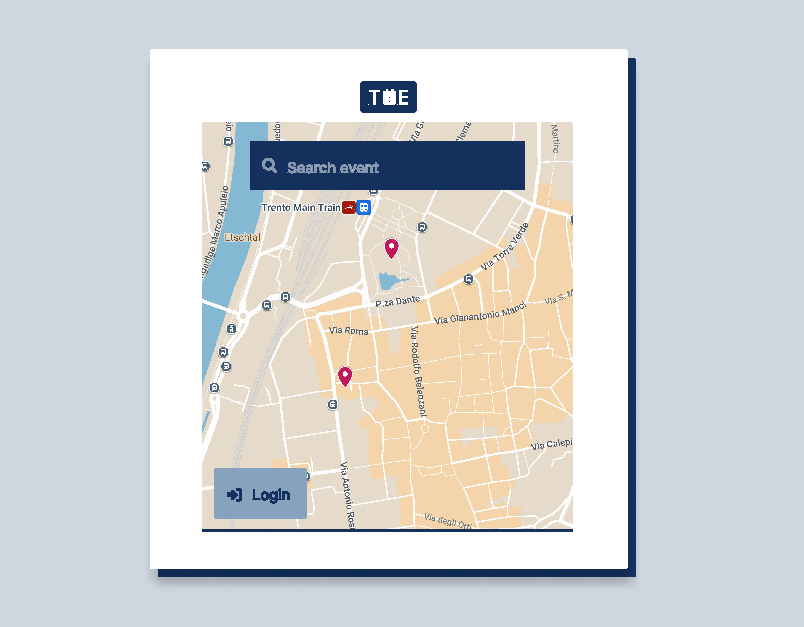
\includegraphics[width=.7\linewidth]{./images/MainPage.pdf}
	\caption{Main page.}
	\label{fig:mainPage}
\end{figure}

In Figura \ref{fig:mainPage} è rappresentata la schermata principale dell'applicazione. Da qui è possibile effettuare la ricerca di eventi senza dover necessariamente effettuare il login.

\begin{figure}[!htb]
	\centering
	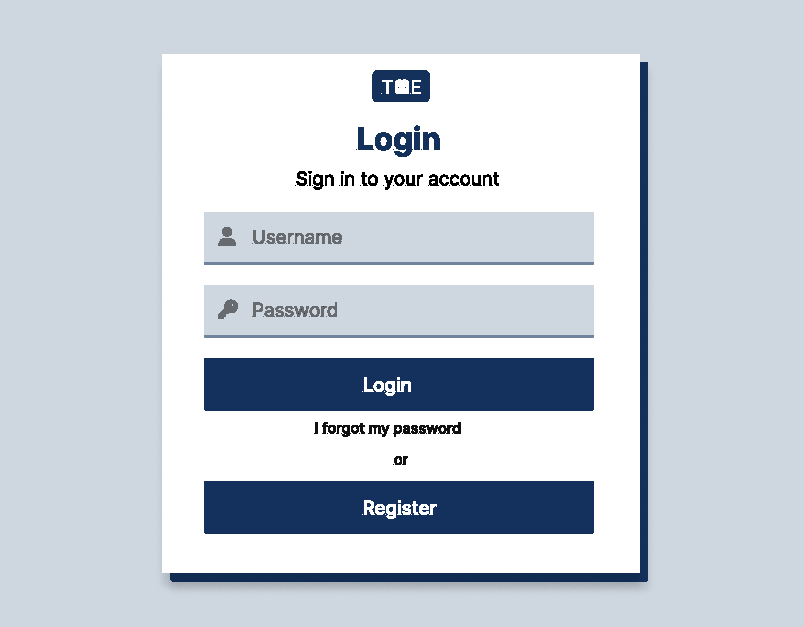
\includegraphics[width=.7\linewidth]{./images/Login.pdf}
	\caption{Login page.}
	\label{fig:login}
\end{figure}


\begin{figure}[!htb]
	\centering
	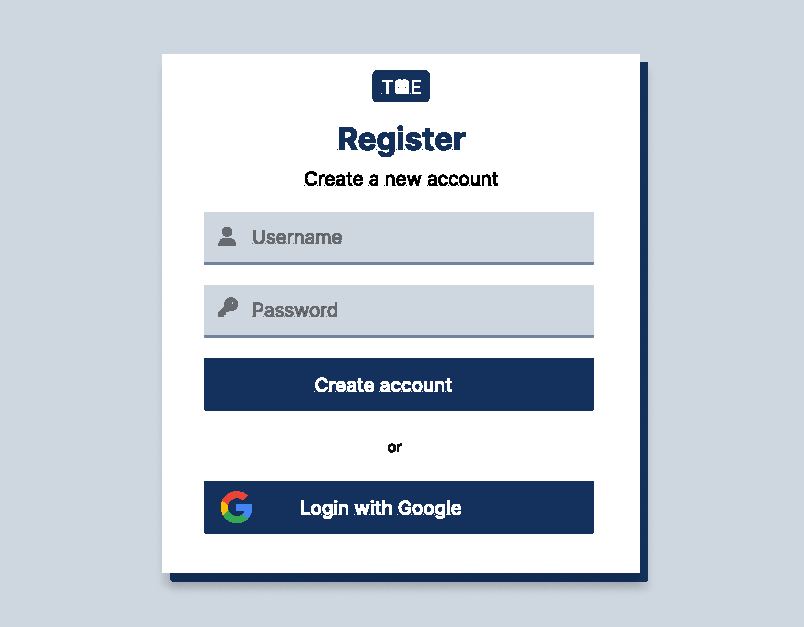
\includegraphics[width=.7\linewidth]{./images/Register.pdf}
	\caption{Register page.}
	\label{fig:register}
\end{figure}



\end{document}